% This is text associated with the open textbook "Open Electromagnetics"
% See immediately below for author, date
% This work is licensed under the Creative Commons Attribution-ShareAlike 4.0 International License. (CC BY SA 4.0) 
% To view a copy of the license, visit http://creativecommons.org/licenses/by-sa/4.0/

%ORB TITLE Displacement Current and Ampere's Law
%ORB AUTHOR 0        # S.W. Ellingson, Virginia Tech (ellingson@vt.edu)
%ORB DATE 20180807   # yyyymmdd
%ORB ABSTRACT Displacement Current and Ampere's Law

\label{m0053_Displacement_Current_Amperes_Law} % <-- Must match name of this file and module directory name.  Don't mess with this!
\index{Ampere's law!general form|(}

In this section, we generalize Ampere's Law, previously encountered as a principle of magnetostatics in Sections~\ref{m0019_Amperes_Law_Magnetostatics} and \ref{m0118_Amperes_Law_Magnetostatics_Integral-to-Differential}.
Ampere's Law states that the current $I_{encl}$ flowing through closed path $\mathcal{C}$ is equal to the line integral of the magnetic field intensity ${\bf H}$ along $\mathcal{C}$.
That is:
%
\begin{equation}   
\oint_{\mathcal{C}}{ {\bf H} \cdot d{\bf l} } = I_{encl}
\label{m0053_fACLI} 
\end{equation}
%
We shall now demonstrate that this equation is unreliable if the current is not steady; i.e., not DC.

First, consider the situation shown in Figure~\ref{m0053_fDC}.
Here, a current $I$ flows in the wire, subsequently generating a magnetic field ${\bf H}$ that circulates around the wire (Section~\ref{m0119_Magnetic_Field_of_a_Long_Wire}).
When we perform the integration in Ampere's Law along any path $\mathcal{C}$ enclosing the wire, the result is $I$, as expected.
In this case, Ampere's Law is working even when $I$ is time-varying. 
%
\begin{figure}
\begin{center}
\pdftooltip{{  % note double braces
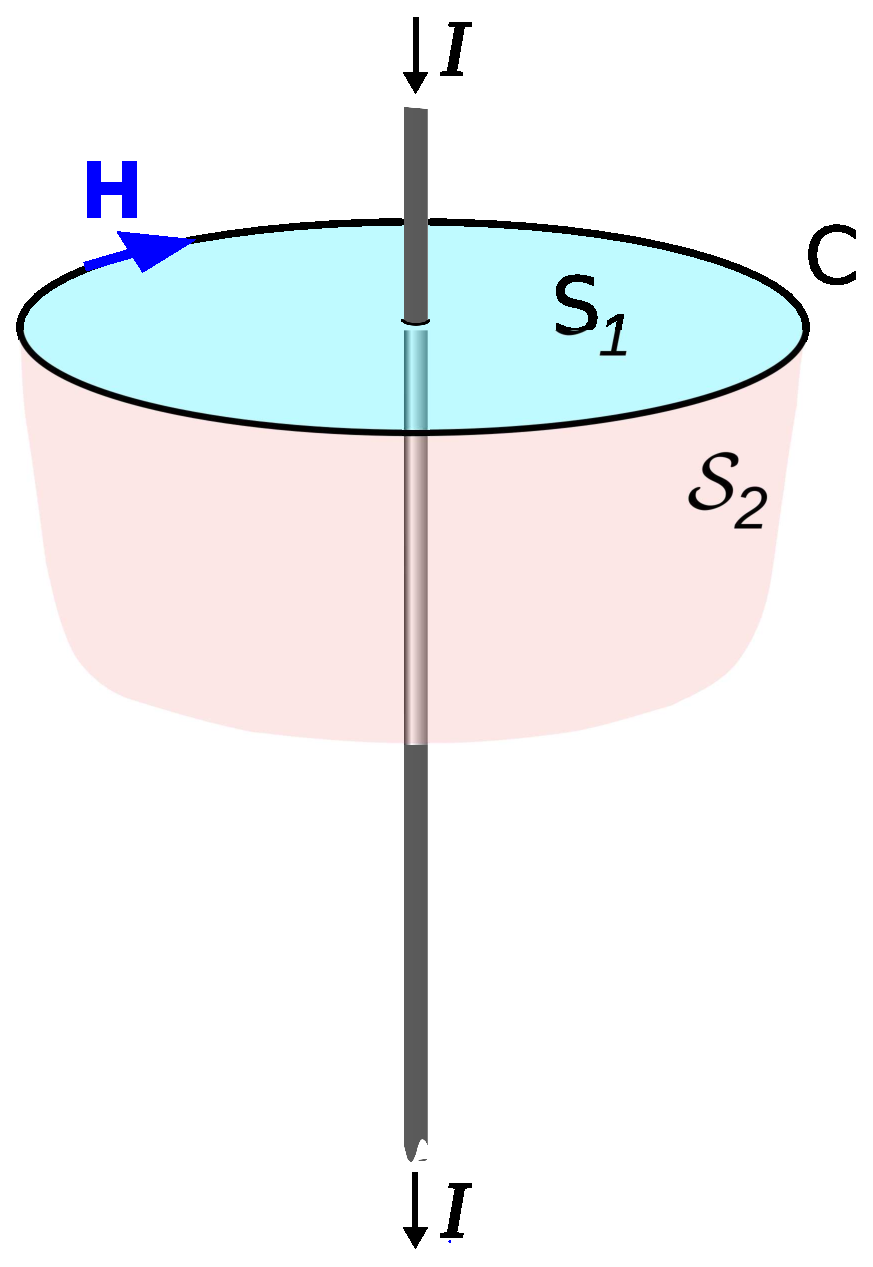
\includegraphics[width=2in]{modules/m0053_fDispCurrent1.eps}
% https://en.wikipedia.org/wiki/File:Displacement_current_in_capacitor.svg
}}{A vertical wire with current I moving down through it. The wire is surrounded by a light blue surface, S sub 1, which is bounded by a closed path, C. The magnetic field intensity, H, is represented by a blue arrow moving in a counterclockwise direction along C. Beneath the surface S sub 1 is a light pink surface, S sub 2, that is the same shape as S sub 1 but extends halfway down the wire, becoming slightly more narrow into a slightly conical shape. }
\end{center} 
\centerline{\scriptsize 
\hyperref[m0053_fDC_Credit]{C.\ Burks} (modified) 
} 
\caption{
\label{m0053_fDC}
Ampere's Law applied to a continuous line of current.
}
\end{figure}

Now consider the situation shown in Figure~\ref{m0053_fAC}, in which we have introduced a parallel-plate capacitor.
In the DC case, this situation is simple.  No current flows, so there is no magnetic field and Ampere's Law is trivially true. 
In the AC case, the current $I$ \emph{can} be non-zero,  but we must be clear about the physical origin of this current.  
What is happening is that for one half of a period, a source elsewhere in the circuit is moving positive charge to one side of the capacitor and negative charge to the other side.
For the other half-period, the source is exchanging the charge, so that negative charge appears on the previously positively-charged side and vice-versa.
Note that at no point is current flowing directly from one side of the capacitor to the other; instead, all current must flow through the circuit in order to arrive at the other plate.
Even though there is no current between the plates, there is current in the wire, and therefore there is also a magnetic field associated with that current.
%
\begin{figure}
\begin{center}
\pdftooltip{{  % note double braces
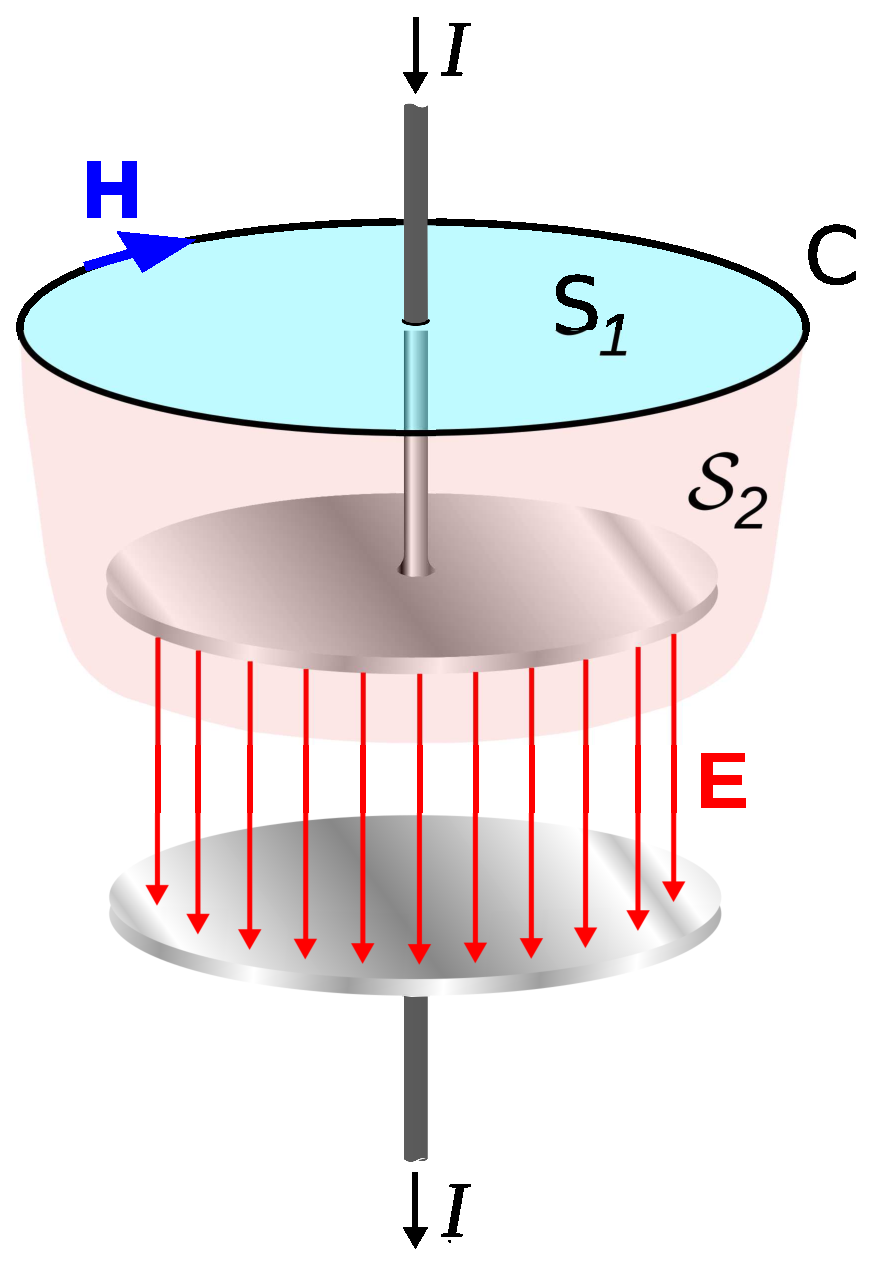
\includegraphics[width=2in]{modules/m0053_fDispCurrent2.eps}
% https://en.wikipedia.org/wiki/File:Displacement_current_in_capacitor.svg
}}{Similar to a previous figure, but features a parallel plate capacitor in the middle of the wire. In the space between the plates are red arrows pointed down in the direction of the electric field, labeled E.}
\end{center} 
\centerline{\scriptsize 
\hyperref[m0053_fAC_Credit]{C.\ Burks} (modified) 
} 
\caption{
\label{m0053_fAC}
Ampere's Law applied to a parallel plate capacitor.
}
\end{figure}

Now we are ready to shine a light on the problem.  
Recall that from Stokes' Theorem 
\index{Stokes' theorem}
(Section~\ref{m0051_Stokes_Theorem}), the line integral over ${\mathcal C}$ is mathematically equivalent to an integral over any open surface ${\mathcal S}$ that is bounded by ${\mathcal C}$.  
Two such surfaces are shown in Figure~\ref{m0053_fDC} and Figure~\ref{m0053_fAC}, indicated as ${\mathcal S}_1$ and ${\mathcal S}_2$.
In the wire-only scenario of Figure~\ref{m0053_fDC}, the choice of ${\mathcal S}$ clearly doesn't matter; any valid surface intersects current equal to $I$.
Similarly in the scenario of Figure~\ref{m0053_fAC}, everything seems fine if we choose ${\mathcal S}={\mathcal S}_1$.
If, on the other hand, we select ${\mathcal S}_2$ in the parallel-plate capacitor case, then we have a problem.  There is no current flowing through ${\mathcal S}_2$, so the right side of Equation~\ref{m0053_fACLI} is zero even though the left side is potentially non-zero.
So, it appears that something necessary for the time-varying case is missing from Equation~\ref{m0053_fACLI}.

To resolve the problem, we postulate an additional term in Ampere's Law that is non-zero in the above scenario.
Specifically, we propose:
%
\begin{equation}   
\oint_{\mathcal{C}}{ {\bf H} \cdot d{\bf l} } = I_c + I_d 
\end{equation}
%
where $I_c$ is the enclosed current (formerly identified as $I_{encl}$) and $I_d$ is the proposed new term.
If we are to accept this postulate, then here is a list of things we know about $I_d$:
%
\begin{itemize}
\item $I_d$ has units of current (A).
\item $I_d=0$ in the DC case and is potentially non-zero in the AC case.  This implies that $I_d$ is the time derivative of some other quantity.
\item $I_d$ must be somehow related to the electric field.
\end{itemize}
%
How do we know $I_d$ must be related to the electric field? This is because the Maxwell-Faraday Equation 
\index{Maxwell-Faraday equation}
(Section~\ref{m0050_Maxwell-Faraday_Equation}) tells us that spatial derivatives of ${\bf E}$ are related to time derivatives of ${\bf H}$; i.e., ${\bf E}$ and ${\bf H}$ are coupled in the time-varying (here, AC) case.  
This coupling between ${\bf E}$ and ${\bf H}$ must also be at work here, but we have not yet seen ${\bf E}$ play a role.  This is pretty strong evidence that $I_d$ depends on the electric field.

Without further ado, here's $I_d$:
%
\begin{equation}   
I_d = \int_{\mathcal{S}} { \frac{\partial {\bf D}}{\partial t} \cdot d{\bf s} }
\end{equation}
%
where ${\bf D}$ is the electric flux density (units of C/m$^2$) and is equal to $\epsilon{\bf E}$ as usual,
and $\mathcal{S}$ is the same open surface associated with $\mathcal{C}$ in Ampere's Law.
Note that this expression meets our expectations:
It is determined by the electric field, it is zero when the electric field is constant (i.e., not time varying), and has units of current.

The quantity $I_d$ is commonly known as \emph{displacement current}.
\index{displacement current}
It should be noted that this name is a bit misleading, since $I_d$ is not a current in the conventional sense.
Certainly, it is not a \emph{conduction} current -- conduction current is represented by $I_c$, and there is no current conducted through an ideal capacitor.
It is not unreasonable to think of $I_d$ as current in a more general sense, for the following reason.  At one instant, charge is distributed one way and at another, it is distributed in another way.  If you define current as a time variation in the charge distribution relative to $\mathcal{S}$ -- regardless of the path taken by the charge -- then $I_d$ is a current.
However, this distinction is a bit philosophical, so it may be less confusing to interpret ``displacement current'' instead as a separate electromagnetic quantity that just happens to have units of current.

Now we are able to write the general form of Ampere's Law that applies even when sources are time-varying.  Here it is:
%
\begin{equation}   
\boxed{
\oint_{\mathcal{C}}{ {\bf H} \cdot d{\bf l} } = I_c + \int_{\mathcal{S}} { \frac{\partial {\bf D}}{\partial t} \cdot d{\bf s} }
}
\label{m0053_eACLI} 
\end{equation}
%
As is the case in the Maxwell-Faraday Equation, most of the utility of Ampere's Law is unleashed when expressed in differential form.
To obtain this form the first step is to write $I_c$ as an integral of over $\mathcal{S}$; this is simply (see Section~\ref{m0101_Current_Distributions}):
%
\begin{equation}   
I_c = \int_{\mathcal{S}} {\bf J} \cdot d{\bf s} 
\end{equation}
%
where ${\bf J}$ is the volume current density (units of A/m$^2$).  So now we have
%
\begin{flalign}   
\oint_{\mathcal{C}}{ {\bf H} \cdot d{\bf l} } &= \int_{\mathcal{S}} {\bf J} \cdot d{\bf s}  + \int_{\mathcal{S}} { \frac{\partial {\bf D}}{\partial t} \cdot d{\bf s} } \nonumber \\
                                              &= \int_{\mathcal{S}} { \left({\bf J}+ \frac{\partial {\bf D}}{\partial t} \right) \cdot d{\bf s} } 
\end{flalign}
%
We can transform the left side of the above equation into a integral over $\mathcal{S}$ using Stokes' Theorem (Section~\ref{m0051_Stokes_Theorem}).
We obtain 
%
\begin{equation}   
\int_{\mathcal{S}} { \left( \nabla \times {\bf H} \right) \cdot d{\bf s}  }  = \int_{\mathcal{S}} { \left({\bf J}+ \frac{\partial {\bf D}}{\partial t} \right) \cdot d{\bf s} } 
\end{equation}
% 
The surface $\mathcal{S}$ on both sides is the same, and we have not constrained $\mathcal{S}$ in any way. $\mathcal{S}$ can be any mathematically-valid open surface anywhere in space, having any size and any orientation.
The only way the above expression can be universally true under these conditions is if the integrands on each side are equal at every point in space.
Therefore: 
%
\begin{equation}   
\boxed{
\nabla \times {\bf H} = {\bf J} + \frac{\partial}{\partial t}{\bf D}
}
\label{m0053_eACLD}
\end{equation}
%
which is Ampere's Law in differential form.

What does Equation~\ref{m0053_eACLD} mean? Recall that the curl of ${\bf H}$ is a way to describe the direction and rate of change of ${\bf H}$ with position.  Therefore, this equation constrains spatial derivatives of ${\bf H}$ to be simply related to ${\bf J}$ and the time derivative of ${\bf D}$ (displacement current).  Said plainly:

%ORB HIGHLIGHT
\begin{mdframed}[backgroundcolor=yellow!20,nobreak=true] 
The differential form of the general (time-varying) form of Ampere's Law (Equation~\ref{m0053_eACLD}) relates the change in the magnetic field with position to the change in the electric field with time, plus current.
\end{mdframed}

As is the case in the Maxwell-Faraday Equation (Section~\ref{m0050_Maxwell-Faraday_Equation}), we see that electric and magnetic fields become coupled at each point in space when sources are time-varying. 

%%%%%%%%%%%%%%%%%%%%%%%%%%%%%%%%%%%%%%

{\bf Additional Reading:}
\begin{itemize}
\item ``\href{https://en.wikipedia.org/wiki/Displacement_current}{Displacement Current}'' on Wikipedia.
\item ``\href{https://en.wikipedia.org/wiki/Ampere's_circuital_law}{Ampere's Circuital Law}'' on Wikipedia.
\item ``\href{https://en.wikipedia.org/wiki/Maxwell's_equations}{Maxwell's Equations}'' on Wikipedia.
\end{itemize}

\index{Ampere's law!general form|)}


